\documentclass[../TDE6_rsf.tex]{subfiles}%

\begin{document}
\section[s]"1"{Obtention d'une équation différentielle}
\QR{%
	\begin{minipage}[t]{0.60\linewidth}
		En utilisant les lois de \textsc{Kirchhoff} en complexes, montrer que la
		tension $u(t)$ est solution de l'équation différentielle
		\[4\tau^2 \dv[2]{u}{t} + 5\tau \dv{u}{t} + u(t) = e(t)
			\qavec
			\tau = RC
		\]
	\end{minipage}
	\hfill
	\begin{minipage}[t]{0.35\linewidth}
		\vspace{0pt}
		\begin{center}
			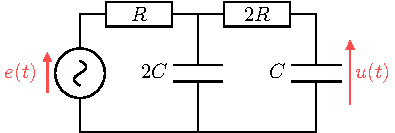
\includegraphics[width=\linewidth]{eqdiff_rcrc_plain}
		\end{center}
	\end{minipage}
}{%
	\noindent
	\begin{isd}
		\begin{center}
			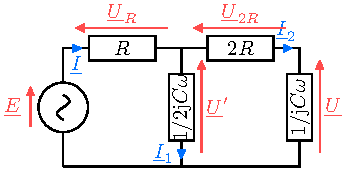
\includegraphics[width=\linewidth]{eqdiff_rcrc_cplx}
		\end{center}
		\tcblower
		On nomme les tensions et intensités dans le circuit, et on utilise la loi des
		nœuds et la loi d'\textsc{Ohm} généralisée~:
		\begin{gather}
			\nonumber
			\xul{I} = \xul{I_1} + \xul{I_2}\\
			\nonumber
			\Lra
			\frac{1}{R}\xul{U_R} = \frac{1}{\Zu_{2C}}\xul{U'} + \frac{1}{\Zu_C}\Uu\\
			\label{eq:ex6}
			\Lra
			\xul{U_R} = 2\jrcw\xul{U'} + \jrcw\Uu
		\end{gather}
	\end{isd}
	On utilise ensuite la loi des mailles à droite et à gauche, donnant
	respectivement~:
	\begin{gather*}
		\xul{U'} = \Uu + 2R\xul{I_2} = \Uu + 2\jrcw\Uu
		\qet
		\xul{U_R} = \Eu - \xul{U'} = \Eu - \Uu - 2\jrcw\Uu
	\end{gather*}
	On regroupe les équations dans \eqref{eq:ex6} et on introduit $\tau
		= RC$~:
	\begin{gather*}
		\Eu - \Uu - 2\jw\tau\Uu = \jw\tau \left( \Uu +
		2\jw\tau\Uu \right) + \jw\tau\Uu\\
		\Lra
		\Eu = \Uu + 5\jw\tau\Uu + 4\tau^2 (\jw)^2\Uu
	\end{gather*}
	En identifiant les puissances de $\jw$ à l'ordre des dérivées pour retourner
	dans le domaine des représentations réelles, on a donc bien
	\begin{gather*}
		\boxed{
			e(t) = u(t) + 5\tau \dv{u}{t} + 4\tau^2 \dv[2]{u}{t}}
	\end{gather*}
}
\end{document}
